\subsection{General description}

The parallel version of ECHAM is based on a domain distribution
approach, i.e.~every processor only handles a limited domain of the
whole globe, and only keeps the respective part of the data. In order
to facilitate the distribution, the whole domain is divided into {\tt
nproca} times {\tt nprocb} domains with {\tt nproca} being the number
of divisions in north-south direction and {\tt nprocb} the number of
divisions in east west direction.  In order to achieve a good load
balance in the shortwave radiation (and chemical reaction)
calculations, each processor treats two parts of the globe, located
opposite to each other. So half of the gridpoints of each processor
will be on the daytime and the other half on the nighttime side on the
globe.

Parts of the calculations within ECHAM are performed in spectral
space. For these calculations the spectral coefficients are
distributed over processors as well. In order to perform the Fourier
and Legendre transformations - which are global operations in
gridpoint and spectral space as well - two further data distributions
are used, named Fourier and Legendre space. The data distributions are
sketched in Figure {\ref{fig.transpose}}, a more detailed discription
is given in Section {\ref{sec.decompose}}.

\begin{figure}[htb]
%\[
%\ifpdf
\centerline{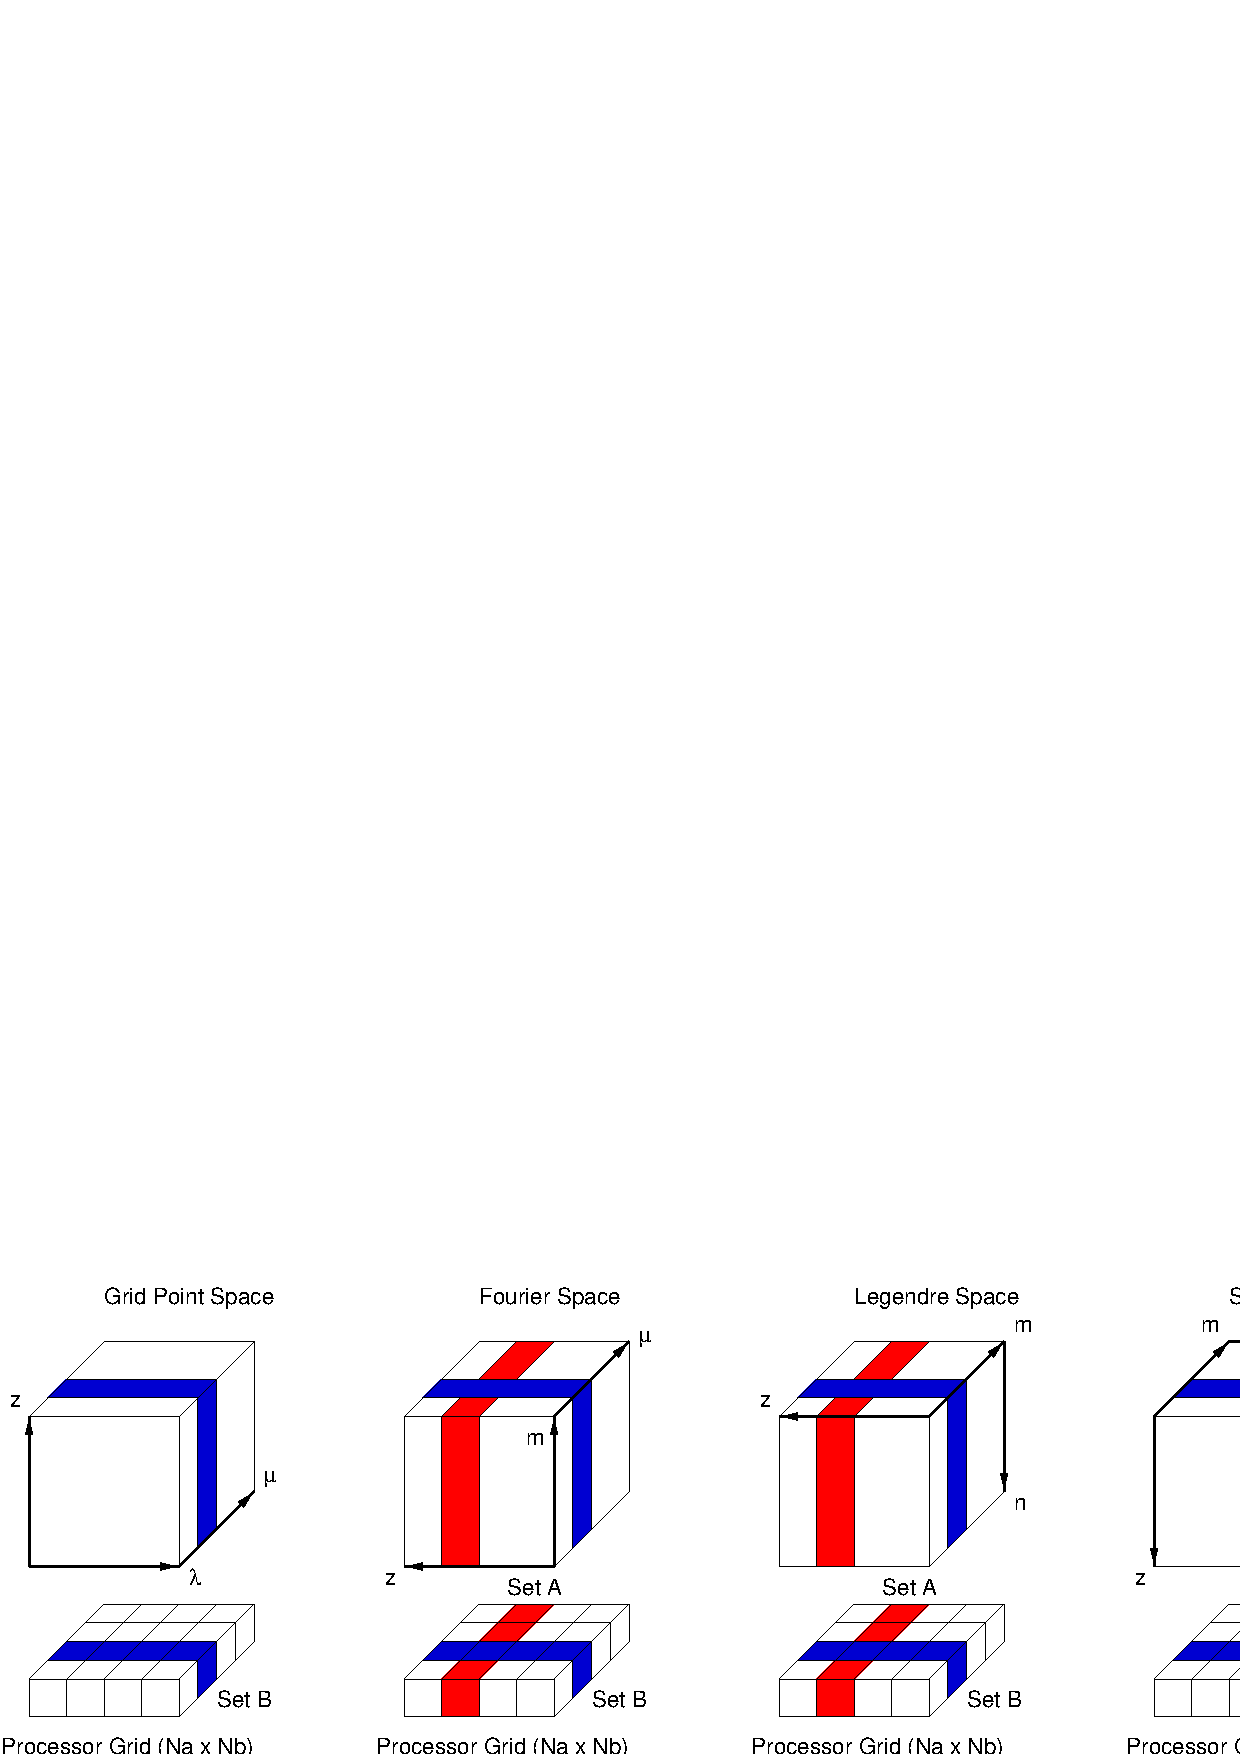
\includegraphics[width=12cm]{guide/transpose.pdf}}
%\else
%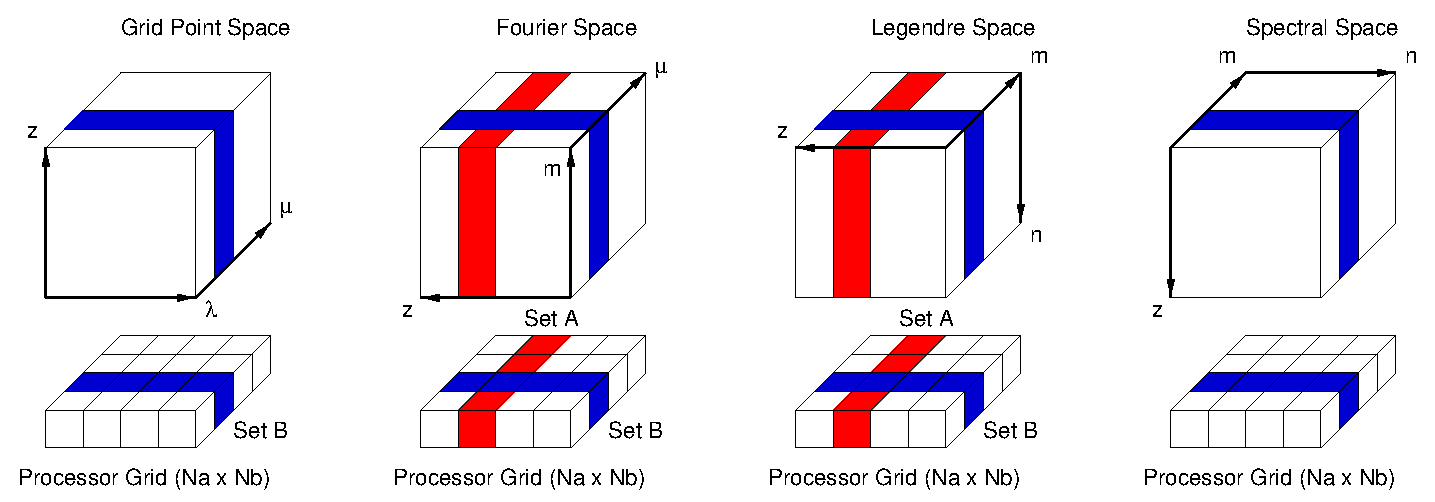
\includegraphics[width=12cm]{guide/transpose.eps}
%\fi
%\]
\caption{Data distribution}
\label{fig.transpose}
\end{figure}

The data transpositions, i.e. the redistribution of data in order to
perform the global Fourier and Legendre transformations are performed
just before and after these transformations. All other calculations
require almost no further communication (besides a few global sums)
because the data required for the operations is present on the
respective processor.  A recipe for writing parallel routines is given
in Section {\ref{sec.recipe}}.


\subsection{Recipe for writing or modifying parallel routines}
\label{sec.recipe}

\subsubsection{Physical parameterizations}

The physical parameterization routines (called from the routines {\tt
gpc} or {\tt physc}) work only on one block of grid cells of
consecutive longitudes. This block can be too short to accomodate all
grid cells of one latitude of it may combine grid cells of more than
one latitude into one block. The length of the block can be chosen
arbitrarily and is called {\tt nproma}. The loop
over the blocks is performed in a higher level routine ({\tt scan1})
and the actual block length 
is passed to the respective subroutines as {\tt kproma}.

``Physics'' computations at different model columns are generally
independent from 
each other and do not require any communication between
processors. Furthermore most computations do not depend on the
absolute location on the globe. If these two conditions are fullfilled
no further action is required for the parallel model version and a
physical parameterization routine may remain unchanged. Loops over the
grid cells in one block are performed by the following statement:
\begin{verbatim}
DO i=1, kproma
  ...
END DO
\end{verbatim}
Special care must be taken if:
\begin{enumerate}
\item The routines are not called within the loop over blocks.

In this case the number of longitudes and latitudes handled by the
processor can be accessed by reference to the components {\tt nglon}
and {\tt nglat} of the variable {\tt local\_decomposition} in module
{\tt mo\_decompose} (cf.{} Section {\ref{sec.decompose.grid}}). A
typical loop over blocks and block elements is given below.  {\tt
dc\%ngpblks} and {\tt dc\%nproma} ({\tt dc\%npromz}) are also used to
specify the 
dimensions of local arrays.
\begin{verbatim}
use mo_decomposition, only: dc => local_decomposition
real(dp) :: xlocal (dc%nproma, dc%ngpblks) ! declare a local array
...
DO j=1, dc%ngpblks-1                  ! loop over local block
  DO i=1, dc%nproma                   ! loop over grid cells in block
    ...
    xlocal (i,j) = 0._dp              ! access a local array
    ...
  END DO
END DO
DO i=1, dc%npromz
   ...
   xlocal (i,dc%ngpblks) = 0._dp
   ...
END DO
\end{verbatim}

\item An index to a global field is required or the absolute position on the
globe must be known.

These conditions are met in the short-wave radiation part, where the
zenith angle of the sun must be calculated, or if the horizontal area
covered by a column must be known, for instance in budget
calculations.

Every processor handles two distinct parts of the domain on opposite
sides of the globe. For this reason the first {\tt dc\%ngpblks/2}
blocks are located on the northern hemisphere whereas the
remaining lines are located on the southern hemisphere.
The local as well as the global
latitude generally runs from North to South, but some of the global
arrays (for instance Gaussian weights) are still stored in so called
ping-pong order (with one latitude line in the northern hemisphere
being followed by the respective latitude line from the southern
hemisphere).

For routines called within {\tt gpc} or {\tt physc} the local latitude
index {\tt jglat} and the global ping-pong index {\tt igprow} are
stored in the module variable {\tt nrow(2)} in module {\tt mo\_control}:
\begin{verbatim}
nrow(1) = igprow ! global ping pong index
nrow(2) = jlat   ! local  index north -> south
\end{verbatim}

\item Global sums are required.

Global sums should be avoided, in order to prevent communication
between processors. In the case that global operations cannot be
avoided, routines to derive global (or zonal) sums may be found in
module {\tt mo\_global\_op} (cf.{} Section\,{\ref{sec.globalop}}).

\item Dependencies between horizontal gridpoints exist.

Dependencies between horizontal gridpoints within the physical
routines should be avoided, in order to prevent communication between
processors. If possible these calculations should be done at locations
in the program where suitable data transpositions have already been
performed or in dedicated routines (for instance in the
semi--Lagrangian transport routine).

\item Input and Output

Input and Output is addressed in Section {\ref{sec.recipe.io}}

\end{enumerate}

\subsubsection{Input/Output}
\label{sec.recipe.io}

Two things must be considered when files are read or written:
\begin{enumerate}
\item 
  In parallel mode, only one processor is allowed to perform I/O. This
  processor will also be called I/O processor.
  The logical variable {\tt p\_parallel\_io} (from {\tt mo\_mpi}) has
  the value {\tt .true.} on the I/O processor only and has the value
  {\tt .false.} on all other processors.
  In single processor mode
  (indicated by a value {\tt .false.} of {\tt p\_parallel}) the data
  is merely read or written.
\item
  The values of variables read by the I/O processor must be communicated to the
  other processors. If all processors are supposed to receive the same
  information the broadcast routine {\tt p\_bcast} (from {\tt
  mo\_mpi}) must be called. In case of two or three dimensional arrays
  each processor only holds the information relevant for its
  subdomain. In this case the I/O must be performed on a global
  variable (generally only allocated on the processor which performs
  I/O) different from the local variable which finally is used for
  computations.  In order to communicate the data to processors in
  gridpoint space the routine {\tt scatter\_gp} from module {\tt
  mo\_transpose} must be called. Similar routines exist in order to
  distribute data in spectral space ({\tt scatter\_sp}) or do gather
  the data from the other processors ({\tt gather\_gp}, {\tt
  gather\_sp}). Generic interfaces are provided for the broadcast
  and gather or scatter routines
  (cf.{} Section\,{\ref{sec.mo-transpose}}) for different data types
  and array dimensions.
\end{enumerate}

Below some examples are given. Note that generally I/O is not
performed directly, but routines are provided for reading and writing
specific formats (Grib, Netcdf).

\begin{enumerate}
\item Read and broadcast some information

The broadcast routine requires {\tt p\_io} as actual parameter in
order to identify the processor which sends the information, i.e.{}
the processor which performs I/O.
\begin{verbatim}
  USE mo_mpi, ONLY: p_parallel, p_parallel_io, p_broadcast, p_io
  IF (p_parallel) THEN
     IF (p_parallel_io) THEN
        READ x
     ENDIF
     CALL p_bcast (x, p_io)
  ELSE
     READ x
  ENDIF
\end{verbatim}
\item Read and scatter some information

In this example {\tt x} is a 3 dimensional field
({\tt kbdim}, {\tt levels}, {\tt ngpblks}, where {\tt kbdim} is the
maximum length of block) which finally stores the local information
on each processor. Information on the data distribution of all
processors is provided in the variable {\tt global\_decomposition} and
must be passed to the scatter and gather routines.
\begin{verbatim}
  USE mo_mpi,       ONLY: p_parallel, p_parallel_io, p_io
  USE mo_transpose, ONLY: scatter_gp
  USE mo_decompose, ONLY: gl_dc => global_decomposition, &
                          dc    => local_decomposition
  REAL, POINTER :: tmp (:,:,:)                ! global read buffer
  REAL          :: x   (dc%nproma, dc%nlev, dc%ngpblks) 
  IF (p_parallel) THEN                        ! in parallel mode:
    NULLIFY(tmp)                       ! nullify global array not used
    IF(p_parallel_io) THEN
      ALLOCATE (tmp(dc%nlon,dc%nlev,dc%nlat)) ! allocate global array used
      READ x                                  ! read information
    ENDIF
    CALL scatter_gp(tmp, x, gl_dc)            ! scatter 
    IF (p_parallel_io) DEALLOCATE (tmp)       ! deallocate global array
  ELSE                                        ! in single processor mode:
     READ x                                   ! merely read  
  ENDIF
\end{verbatim}
\item Gather and write some information

This example is very similar to the previous one.
\begin{verbatim}
  USE mo_mpi,       ONLY: p_parallel, p_parallel_io, p_io
  USE mo_transpose, ONLY: gather_gp
  USE mo_decompose, ONLY: gl_dc => global_decomposition, &
                          dc    => local_decomposition
  REAL, POINTER :: tmp (:,:,:)                ! global read buffer
  REAL          :: x   (dc% nglon, dc% nlev, dc% nglat) 
  IF (p_parallel) THEN                        ! in parallel mode:
    NULLIFY(tmp)                       ! nullify global array not used
    IF(p_parallel_io) THEN
      ALLOCATE (tmp(dc%nproma,dc%nlev,dc%ngpblks)) ! allocate 
                                       !global array used
    ENDIF
    CALL gather_gp(tmp, x, gl_dc)             ! gather 
    IF(p_parallel_io) THEN
      WRITE x                                 ! write information
      DEALLOCATE (tmp)                        ! deallocate global array
    ENDIF
  ELSE                                        ! in single processor mode:
     WRITE x                                  ! merely write
  ENDIF
\end{verbatim}
\end{enumerate}

%\subsection{Message Passing Interface (mo\_mpi)}
% to be added in a later version

\subsection{Decomposition (mo\_decompose)}
\label{sec.decompose}

The decomposition is handled by the module {\tt mo\_decompose} which
is described in this section.

The domain decomposition is performed by a call to the routine {\tt
decompose} with the following parameters:

\begin{description}
\item{\tt global\_dc}\\
  Derived decomposition table (output).
\item{\tt nlat, nlon, nlev}\\
  These parameters determine the size of the global domain: {\tt nlat}
  is the number of latitudes (which must be even), {\tt nlon} is the
  number of longitudes and {\tt nlev} is the number of levels.
\item{\tt nm, nn, nk}\\
  These parameters give the number of wavenumbers in spectral
  space. Currently only triangular truncation is allowed with {\tt
  nm = nn = nk}.
\item{\tt nproca, nprocb}\\
  Following the ideas of the Integrated Forecast System (IFS) of the
  European Centre of Midium--Range Weather Forcast (ECMWF) the
  total domain is covered by {\tt nproca} times {\tt nprocb}
  processors. In Gridpoint space the domain is divided into {\tt
  nprocb} subdomains in east-west direction and 2 times {\tt nproca}
  subdomains in north-south directions. Details are given below in the
  subsections of this paragraph.

  The default decomposition may be modified by the following optional
  parameters:
\item{\tt norot}\\
  In order to improve load balancing in the shortwave radiation part
  half of the gridpoints of each processor should be exposed to the
  sun whereas the other half should be located at the nocturnal side
  of the globe. Thus each processor handles two subdomains on opposite
  sides of the globe. Actually the two domains must consist of
  latitude rows with the same absolute values of latitudes, but with
  opposite sign. The longitude values in the southern domain are
  rotated by 180 degree with respect to the corresponding gridpoints
  in the northern domain.
  Setting this optional parameter to {\tt .true.} the southern domain is
  not rotated. If the code runs on one processor this results in a
  continuous global domain as in the serial program version.
\item{\tt lfull\_m}\\
  Setting this optional parameter to {\tt .true.} ensures that the
  decomposition in spectral space does not spread wavenumbers with the
  same longitudinal wavenumber $m$ over different processors. This
  option is not recommended because it decreases load balance in
  spectral space.
\item{\tt debug}\\
  Setting this optional parameter to {\tt .true.} runs a second
  copy
  of the model using one additional processor so that ${\tt
  nproca}\times{\tt nprocb}+1$ processors are required in this
  case. Furthermore it is assumed that {\tt norot=.true.} for this
  additional run so that the decomposition corresponds with that of
  the original serial version.

  The values of the variables of the two model copies are compared
  at certain breakpoints and further tests for equality of
  corresponding variables can be inserted at any time of program
  execution. This is the most rigorous test of the parallel version.

  A value {\tt .true.} of the logical module variable {\tt
  debug\_parallel} indicates that the parallel test mode is enabled.
\end{description}

Decomposition information is stored in the module variables 
{\tt global\_decomposition} and {\tt local\_decomposition} of derived
type {\tt pe\_decomposed}. The elements of the array {\tt
global\_decomposition} describe the decomposition for each processor.
The scalar type {\tt local\_decomposition} holds the decomposition of
the actual processor.

The data type {\tt pe\_decomposed} described in the subsection below
holds the decomposition information for a single processor.

\subsubsection{Information on the whole model domain}

The following components of data type {\tt pe\_decomposed} have the
same contents for all processors of the model:

\begin{description}
\item{\tt nlon}: number of longitudes of the global domain.
\item{\tt nlat}: number of latitudes of the global domain.
\item{\tt nlev}: number of levels of the global domain.
\item{\tt nm}:   
maximum wavenumber used. Only triangular truncation is supported.

The following components depend on {\tt nm}:
\item{\tt nnp(m+1)}: 
number of spectral coefficients for each longitudinal wavenumber $m$,
$m=0,nm$
\item{\tt nmp(m+1)}:
displacement of the first point of m-columns within the array storing
the spectral coefficients. Actually {\tt nmp(1)=0} and {\tt
nmp(nm+2)=} last index of the array storing the spectral
coefficients. The actual number of coefficiens is $2\times nmp(nm+2)$
because 2 coefficients are stored for each wavenumber.
\end{description}

\subsubsection{Information valid for all processes of a model instance}
\label{sec.decompose.grid}

The following components of data type {\tt pe\_decomposed} have the
same contents for all processors of each instance of the model:

\begin{description}
\item{\tt nprocb}:
number of processors for the dimension that counts longitudes
\item{\tt nproca}:
number of processors for the dimension that counts latitudes
\item{\tt d\_nprocs}:
number of processors used in the model domain $nproca\times nprocb$.
\item{\tt spe, epe}:
Index number of first and last processor which handles this model domain.
\item{\tt mapmesh(ib,ia)}:
array mapping from a logical 2-d mesh to the processor index numbers
within the decomposition table {\tt global\_decomposition}. $ib=1,nprocb$;
$ia=1,nproca$.
\end{description}

\subsubsection{General Local Information}

The contents of the remaining components of data type {\tt
pe\_decomposed} is specific for each processor.

\begin{description}
\item{\tt pe}:
processor identifier. This number is used in the {\tt mpi} send and
receive routines.
\item{\tt set\_b}:
index of processor in the direction of logitudes. This number
determines the location within the array {\tt mapmesh}. processors
with ascending numbers handle subdomains with increasing longitudes
(i.e. from west to east).
\item{\tt set\_a}:
index of processor in the direction of latitudes. This number
determines the location within the array {\tt mapmesh}. Processors
with ascending numbers handle subdomains with decreasing values of
absolute latitudes (i.e. from the pole to the equator within each
hemisphere).
\end{description}

\subsubsection{Grid space decomposition}

In grid space longitudes and latitudes are spread over
processors. Each processor handles all levels of a model column.

\begin{description}
\item{\tt nglat, nglon}:
number of latitudes and longitudes in grid space handled by this processor.
\item{\tt glats(1:2), glate(1:2)}:
start and end values of global latitude indices. 
\item{\tt glons(1:2), glone(1:2)}:
start and end values of global of longitude indices.  Each processor
handles two subdomains located on opposite sides of the globe. The
first elements {\tt 1:nglat/2} of array dimensions indexing latitudes
correspond to global latitude indices {\tt glats(1):glate(1)}.  The
last elements {\tt nglat/2+1:nglat} correspond to global latitude
indices {\tt glats(2):glate(2)}.  Both, local and global latitude
indices run from north to south.  Elements
$e(i,j),i=1:nglon,j=1:nglat/2$ of a local array correspond to elements
$g(k,l),k=glons(1), glone(1),l=glats(1):glate(1)$ of the respective
global array.
\item{\tt glat(1:nglat)}:
global latitude index.
\item{\tt glon(1:nglon)}:
offset to global longitude index.  These components facilitate
indexing of global arrays. Elements $e(i,j),i=1:nglon,j=1:nglat/2$ of
a local array correspond to elements $g(glat(i),+glon(i)+j)$ of the
respective global array.
\end{description}

\subsubsection{Fourier space decomposition}

In order to perform the Fourier transformation, the arrays are
redistributed so that each processor holds all longitudes or Fourier
components. Latitudes are spread over processors as in grid
space. Additionally the levels are distributed.

\begin{description}
\item{\tt nflat, nflev}:
number of latitudes and levels on this processor.
\item{\tt nflevp1}:
number of levels plus one on this processor. If global arrays hold
{\tt nlev+1} elements per column they require {\tt nflevp1} on this
processor. {\tt nflevp1} is equal to {\tt nflev+1} if the last level
is handled by this processor, otherwise {\tt nflevp1} is equal to {\tt
nflev}.
\item{\tt flats(2), flate(2)}:
start and end values of latitudes indices. As in grid space 2
subdomains located on the northern and southern hemisphere are
handled.
\item{\tt flevs, fleve}:
start and end values of levels. The elements $e(k),k=1,nflevp1$ of a
local array correspond to elements $g(l),l=flevs:fleve$ of the
respective global array.
\item{\tt lfused}:
{\tt .true.} if this processor is used in Fourier space.
\end{description}

\subsubsection{Legendre space decomposition}

In order to perform the Legendre transformation, the arrays are
redistributed so that each processor holds all latitudes or spectral
coefficients for a given longitudinal wavenumber. Levels are spread
over processors as in Fourier space. Additionally the longitudinal
wavenumbers are distributed.

Row of PEs with same set\_a:
\begin{description}
\item{\tt nlm}:
number of local longitudinal wave numbers m handled by this processor.
\item{\tt lm(1:nlm)}:
actual longitudinal wave numbers handled by this processor.
\item{\tt lnsp}:
number of complex spectral coefficients handled by this processor.
\item{\tt nlmp(1:nlm)}:
displacement of the first coefficient of columns (with same
longitudinal wave number) within a globally indexed array (as described
by components {\tt nm}, {\tt nnp}, {\tt nmp}).
\item{nlnp(1:nlm)}:
number of points on each column with same longitudinal wave number m.
\item{nlnm0}:
number of coefficients with longitudinal wave number m=0 on this processor.
\end{description}

Column of PEs with same set\_b:
\begin{description}
\item{\tt nllev, nllevp1}:
number of levels (+1) handled by this processor as in Fourier space.
\item{\tt llevs, lleve}:
start and end values of level indices as in Fourier space.
\end{description}

\subsubsection{Spectral space decomposition}

For spectral computations the arrays are redistributed so that each
processor holds all levels for a given spectral
coefficient. Longitudinal wavenumbers are spread over processors as in
Legendre space. Remaining spectral coefficients are spread over
processors.

\begin{description}
\item{\tt snsp, snsp2}:
number of spectral coefficients handled by this processor and number
of coefficients multiplied by 2.
\item{\tt ssps, sspe}:
first and last spectral coefficient with respect to the ordering in
Legendre space.
\item{\tt lfirstc}:
true, if first global coefficient (m=0,n=0) resides on this processor.
\item{\tt ifirstc}:
location of first global coefficient on this processor.
\item{\tt np1(1:snsp)}:
value of (n+1) for all coefficients of this processor.
\item{\tt mymsp(1:snsp)}:
value of m for all coefficients of this processor.
\item{\tt nns}:
number of different n-values for this processor.
\item{\tt nindex(1:nns)}:
values of (n+1) different n-values for this processor.
\item{\tt nsm}:
number of longitudinal wavenumbers per processor.
\item{\tt sm (1:nsm)}:
actual longitudinal wave numbers handled by this processor.
\item{\tt snnp(1:nsm)}:
number of n coefficients per longitudinal wave number m.
\item{\tt snn0(1:nsm)}:
first coefficient n for a given m.
\item{\tt nsnm0}:
number of coefficients with m=0 on this processor.
\end{description}

\subsection{Gather, Scatter and Low Level Transposition Routines 
(mo\_transpose)}
\label{sec.mo-transpose}

The module {\tt mo\_transpose} holds the routines to scatter global
fields (after input) among the processors, to gather distributed
fields from the processors (for output and debug purposes) and to
perform the transpositions between the different decompositions (grid,
Fourier, Legendre and spectral space). 

\subsubsection{Gather and Scatter routines (gather\_xx, scatter\_xx)}

Generic interfaces are defined for specific routines to act on arrays
of different rank (for 3-D atmospheric fields, 2-D surface fields,
etc.\ ). Arrays of rank 4 are supported in order to handle arrays
allocated in memory buffer. The actual representation (2-D, 3-D) is
derived from the shape of the rank 4 arrays or rank 3 arrays.

All scatter and gather routines have a similar interface:

\begin{description}
\item{\tt subroutine scatter\_xx (gl, lc, gl\_dc)}
\item{\tt subroutine gather\_xx (gl, lc, gl\_dc, [source])}
\end{description}

The postfix {\tt xx} is one of {\tt gp}, {\tt ls}, {\tt sa} or {\tt
sp} and denotes the space to scatter/gather to/from.

The parameter {\tt gl} is a pointer of rank 1 to 4 pointing to the
global array. {\tt gl} needs to be allocated only on the processor
which performs i/o.

The parameter {\tt lc} is an array of the same rank as {\tt gl}
holding the distributed array.

The parameter {\tt gl\_dc} holds the global decomposition table.

All scatter routines distribute a global array from the i/o processor
to the decomposed arrays of all processors, including itself.

The gather routines have an optional parameter {\tt source} in order
to gather fields from different model copies run in parallel for
debug purposes. {\tt source} may have one of the following values:
\begin{description}
\item{\tt -1:} 
gather from all processors. If more than one model copy is run,
the result depends on the actual I/O processor within the
global decomposition table.
\item{\tt 0:}
gather from the i/o processor only. If more than one model copy is
run this is the processor which performs calculations on the whole
model domain.
\item{\tt 1:}
gather from all processors besides the I/O processor. If more than one
model copy is run these processors perform the parallel
calculations on the distributed domain.
\item{\tt not present:} 
The effect is the same as if {\tt source} had the value of the
variable {\tt debug\_parallel} in {\tt mo\_decompose}.
\end{description}

The shape of the arrays {\tt gl} may be one of the following:

\begin{description}
\item{\tt scatter\_gp, gather\_gp}: (grid space)

\begin{tabular}{llll|l}
(nlon,&nlev,&ntrac,&nlat)&3D tracer fields\\
\hline
(nlon,&nlev,&nlat,&1)    &3D gridpoint field\\
(nlon,&nlev,&nlat)&      &\\
\hline
(nlon,&nlat,&1,&1)       &2D surface field\\
(nlon,&nlat,&1)&&\\
(nlon,&nlat)&&&\\
\end{tabular}

{\tt nlon}, {\tt nlat} are the number of longitudes and latitudes of
the global field {\tt gl} as specified by the respective components of
{\tt local\_decomposition}. {\tt nlev}, {\tt ntrac} are arbitrary
numbers of vertical 
levels and tracers.  {\it If more longitudes are passed only {\tt
nlon} or {\tt nglon} longitudes are scattered/gathered.}

\item{\tt scatter\_sp, gather\_sp}: (spectral space)

\begin{tabular}{llll|l}
(nlev,&2,&nsp,&1)& full spectral field\\
(nlev,&2,&nsp)&  & \\
\hline
(nlev,&nnp1,&1,&1)& spectral array with \\
(nlev,&nnp1,&1)&  & m=0 coefficients only \\
(nlev,&nnp1)&  &  & (zonal mean in grid space) \\
\end{tabular}

The global field {\tt gl} has {\tt nsp} spectral coefficients or {\tt
nnp1} coefficients for the zonal wavenumber m=0 only as specified by
the respective components of {\tt local\_decomposition}.  The
corresponding decomposed field {\tt lc} has {\tt snsp} spectral
coefficients or {\tt nsnm0} coefficients for the zonal wavenumber m=0
only.  {\tt nlev} is an arbitrary number of vertical levels.  The
second index is 2 because 2 coefficients are stored for each
wavenumber.

\item{\tt scatter\_sa, gather\_sa}: (symmetric/assymetric Fourier components)

\begin{tabular}{llll|l}
(nlev,&2,&nm+1,&nhgl)& full Fourier transformed field\\
\hline
(nlev,&nhgl,&1,&1)& Fourier transformed field (m=0 only)\\
(nlev,&nhgl)&  &  & (zonal mean in grid space)\\
\end{tabular}

For reasons of computational efficiency, Legendre transformation is
performed on symmetric and asymmetric (with respect to the equator)
fields seperately. The symmetric/asymmetric Fourier components are
input to the Legendre transform (output of the inverse
transform). Thus, the decomposition of these fields corresponds to
Legendre space, i.e.\ vertical levels and zonal wavenumbers are spread
over processors.

The global field {\tt gl} has {\tt nm+1} zonal wavenumbers and {\tt
nlev} or {\tt nlev+1} vertical levels as specified by the respective
components of {\tt local\_decomposition}.  The corresponding
decomposed field {\tt lc} has {\tt nlm} zonal wavenumbers and {\tt
nllev} or {\tt nllevp1} vertical levels. {\tt nhgl=nlat/2} is half of the
number of Gaussian latitudes. The second index of the full fields is 2
because 2 coefficients are stored for each wavenumber.

\item{\tt scatter\_ls, gather\_ls}: (Legendre space)

Scatter and gather routines to/from Legendre space are used for
debugging purposes only. 

\begin{tabular}{llll|l}
(2*(nm+1),&nlev,&nlat,&nvar)& Fourier components, (gather routine
only)\\
\hline
(nlev,&2,&nsp)&& full spectral field\\
\hline
(nlev,&nnp1)&&& spectral field with m=0 only\\
\end{tabular}

Global Fourier transformed fields (in Legendre space distribution)
have {\tt 2*(nm+1)} spectral coefficients and {\tt nlev} or {\tt
nlev+1} vertical levels as specified by the respective components of
{\tt local\_decomposition}. Global spectral fields have {\tt nsp}
spectral wavenumbers or {\tt nnp1} coefficients for m=0 only. The
corresponding decomposed field {\tt lc} has {\tt nlm} zonal
wavenumbers or {\tt lnsp} complex spectral coefficients and {\tt
nllev} or {\tt nllevp1} vertical levels. {\tt nlat} is the number of
latitudes and {\tt nvar} an arbitrary number of variables.

\end{description}

\subsubsection{Transposition routines (tr\_xx\_yy)}

The general interface of the transpose routines is:

{\tt subroutine tr\_xx\_yy (gl\_dc, sign, xxfields.., yyfields..)}\\
{\tt\quad TYPE (pe\_decomposed) :: gl\_dc}\quad decomposition table\\
{\tt\quad INTEGER :: sign}\quad direction of transposition:  
1: xx$-\!\!\!>$yy, -1: xx$<\!\!\!-$yy\\
{\tt\quad REAL :: xxfields}\quad fields in $xx$-space\\
{\tt\quad REAL :: yyfields}\quad fields in $yy$-space

With $xx$, $yy$ being one of {\tt gp} (gridpoint space), {\tt ls}
(Legendre space), or {\tt sp} (spectral space).  The shape of the
array arguments {\tt xxfields}, {\tt yyfields} depends on the data
structure in the respective spaces. The specific interfaces are as
follows:

\begin{verbatim}
SUBROUTINE tr_gp_fs (gl_dc, sign, gp1, gp2, gp3, gp4, gp5, gp6, gp7,&
                     sf1, sf2, sf3, zm1, zm2, zm3, fs, fs0)
!
! transpose
!   sign= 1 : grid point space  -> Fourier space
!   sign=-1 : grid point space <-  Fourier space
! 
!
TYPE (pe_decomposed) ,INTENT(in)     :: gl_dc  (:)       ! decomposition
INTEGER              ,INTENT(in)     :: sign             ! 1:gp>fs; -1:gp<fs
REAL                 ,INTENT(inout)  :: gp1    (:,:,:)   ! gridpoint space 3d
                                        ...
REAL                 ,INTENT(inout)  :: gp7    (:,:,:)   ! 
REAL ,OPTIONAL       ,INTENT(inout)  :: sf1    (:,:)     ! gridpoint space 2d
REAL ,OPTIONAL       ,INTENT(inout)  :: sf2    (:,:)     ! gridpoint space 2d
REAL ,OPTIONAL       ,INTENT(inout)  :: sf3    (:,:)     ! gridpoint space 2d
REAL ,OPTIONAL       ,INTENT(inout)  :: zm1    (:,:)     ! zonal mean
REAL ,OPTIONAL       ,INTENT(inout)  :: zm2    (:,:)     ! zonal mean
REAL ,OPTIONAL       ,INTENT(inout)  :: zm3    (:,:)     ! zonal mean
REAL                 ,INTENT(inout)  :: fs     (:,:,:,:) ! Fourier space
REAL ,OPTIONAL       ,INTENT(inout)  :: fs0    (:,:,:)   ! zonal mean, Four.
\end{verbatim}

\begin{verbatim}
SUBROUTINE tr_fs_ls (gl_dc, sign, fs, ls, fs0, ls0)
!
! transpose
!   sign= 1 : Fourier space  -> Legendre space
!   sign=-1 : Fourier space <-  Legendre space
!
TYPE (pe_decomposed) ,INTENT(in)     :: gl_dc  (:)       ! decomposition
INTEGER              ,INTENT(in)     :: sign             ! 1:fs>ls; -1:gs<ls
REAL                 ,INTENT(inout)  :: fs   (:,:,:,:)   ! fs
REAL                 ,INTENT(inout)  :: ls   (:,:,:,:)   ! ls
REAL ,OPTIONAL       ,INTENT(inout)  :: fs0  (:,:,:)     ! fs, zonal means
REAL ,OPTIONAL       ,INTENT(inout)  :: ls0  (:,:,:)     ! ls, zonal means
\end{verbatim}

\begin{verbatim}
SUBROUTINE tr_ls_sp (gl_dc, sign, ls1, sp1, ls2, sp2, ls3, sp3, ls0, sp0)
!
! transpose
!   sign= 1 : Legendre space  -> spectral space
!   sign=-1 : Legendre space <-  spectral space
!
TYPE (pe_decomposed) ,INTENT(in)     :: gl_dc (:)     ! decomposition
INTEGER              ,INTENT(in)     :: sign          ! 1:ls&gtsp; -1:ls&ltsp
REAL                 ,INTENT(inout)  :: ls1   (:,:,:) ! Legendre space 
REAL                 ,INTENT(inout)  :: sp1   (:,:,:) ! spectral space
                                        ...
REAL                 ,INTENT(inout)  :: ls3   (:,:,:) ! Legendre space
REAL                 ,INTENT(inout)  :: sp3   (:,:,:) ! spectral space
REAL ,OPTIONAL       ,INTENT(inout)  :: ls0   (:,:)   ! Legendre (m=0 only)
REAL ,OPTIONAL       ,INTENT(inout)  :: sp0   (:,:)   ! spectral (m=0 only)
\end{verbatim}

\subsection{High Level Transposition Routines (mo\_call\_trans)}
\label{sec.mo_call_trans}

The routines in module {\tt mo\_call\_trans} gather the fields to be
transposed from the respective modules and pass them as actual
parameters to the routines which finally perform the transformations
(defined in module {\tt mo\_transpose}). 
If ECHAM is run in test mode, the
correctness of the parallel implementation is tested by calling the
respective routines for the ingoing and outgoing parameters.
Test routines are also provided for the content of some buffers.

The fields involved in the
transformation and test routines are listed below.

\begin{center}
\begin{tabular}{|ll|}
\hline
subroutine & spectral\_to\_legendre \\
\hline
Input : & from module mo\_memory\_ls (Legendre space) \\
ld & \\
ltp & \\
lvo & \\
lu0 & \\
\hline
Output :& to module mo\_memory\_sp (spectral space) \\
sd & \\
stp & \\
svo & \\
su0 & \\
\hline
\end{tabular}

\begin{tabular}{|ll|}
\hline
subroutine & legendre\_to\_fourier\\ \hline
Input : & from module mo\_buffer\_fft (Legendre space)\\
fftl & buffer for 2D and 3D fields \\
lbm0 & buffer for zonal means (m=0) \\
\hline
Output :& to module mo\_buffer\_fft (Fourier space)\\
fftz & buffer for 2D and 3D fields \\
fbm0 & buffer for zonal means (m=0) \\
\hline
\end{tabular}

\begin{tabular}{|ll|}
\hline
subroutine & fourier\_to\_gridpoint\\ \hline
Input : & from module mo\_buffer\_fft (Fourier space)\\
fftz & buffer for 2D and 3D fields \\
fbm0 & buffer for zonal means (m=0) \\
\hline
Output :& to module mo\_scan\_buffer (gridpoint space)\\
d\_scb & \\
t\_scb & \\
u\_scb & \\
v\_scb & \\
vo\_scb & \\
dtm\_scb & \\
dtl\_scb & \\
alps\_scb & \\
dalpsl\_scb & \\
dalpsm\_scb & \\
u0\_scb & \\
du0\_scb & \\
ul\_scb & \\
\hline
\end{tabular}

\begin{tabular}{|ll|}
\hline
subroutine & gridpoint\_to\_fourier\\ \hline
Input : & from module mo\_scan\_buffer (gridpoint space)\\
rh\_scb & \\
dm\_scb & \\
vom\_scb & \\
vol\_scb & \\
u0\_scb & \\
du0\_scb & \\
ul\_scb & \\
\hline
Input : & from module mo\_memory\_g1a (gridpoint space)\\
alpsm1 & \\
dm1 & \\
tm1 & \\
vom1 & \\
\hline
Output :& to module mo\_buffer\_fft (Fourier space)\\
fftz & buffer for 2D and 3D fields \\
fbm0 & buffer for zonal means (m=0) \\
\hline
\end{tabular}

\begin{tabular}{|ll|}
\hline
subroutine & fourier\_to\_legendre\\ \hline
Input : & from module mo\_buffer\_fft (Fourier space)\\
fftz & buffer for 2D and 3D fields \\
fbm0 & buffer for zonal means (m=0) \\
\hline
Output :& to module mo\_buffer\_fft (Legendre space)\\
fftl & buffer for 2D and 3D fields \\
lbm0 & buffer for zonal means (m=0) \\
\hline
\end{tabular}

\begin{tabular}{|ll|}
\hline
subroutine & legendre\_to\_spectral\\ \hline
Input : & from module mo\_memory\_ls (Legendre space) \\
ld & \\
ltp & \\
lvo & \\
lu0  & \\
\hline
Output :& to module mo\_memory\_sp (spectral space) \\
sd & \\
stp & \\
svo & \\
su0 & \\
\hline
\end{tabular}

\begin{tabular}{|ll|}
\hline
subroutine & test\_memory\_f (text) \\ \hline
Test : & module mo\_memory\_f \\
f & \\
\hline
\end{tabular}

\begin{tabular}{|ll|}
\hline
subroutine & test\_memory\_gp (text)\\ \hline
\hline
\end{tabular}

\begin{tabular}{|ll|}
\hline
subroutine & test\_scan\_buffer (gp, text)\\ \hline
\hline
\end{tabular}

\begin{tabular}{|ll|}
\hline
subroutine & test\_row\_buffer (j, text)\\ \hline
& \\
\hline
\end{tabular}
\end{center}

%\subsection{Module containing subprograms for testing ({\tt mo\_test\_trans})

\subsection{Global operations ({\tt mo\_global\_op})}\label{sec.globalop}

In this module, subprograms are collected that perform global
operations on 2--d and 3--d fields like the calculation of global or
zonal mean values. Any global operation needs communication between
the processors. Even if integrals are split into integrals over the
domain that is present on each processor and the summation over all
processors, the global operation subroutines slow down the \echam{}
program the more the more processors are used in a simulation. For
this performance reason, it is highly recommended to reduce global
operations to a strict minimum in \echam{} and to perform such
operations in the postprocessing step that can be performed in
parallel to a longer simulation.

%\subsection{Semilagrangian transport}
